\section{Triage}
En esta sección daremos a conocer el camino que recorre la aplicación para cargar los síntomas del paciente.

\subsection{Pantalla inicial de Triage}
La pantalla inicial de Triage (como podemos ver en la figura \ref{fig:triage_inicial}) 
\begin{figure}
\centerline{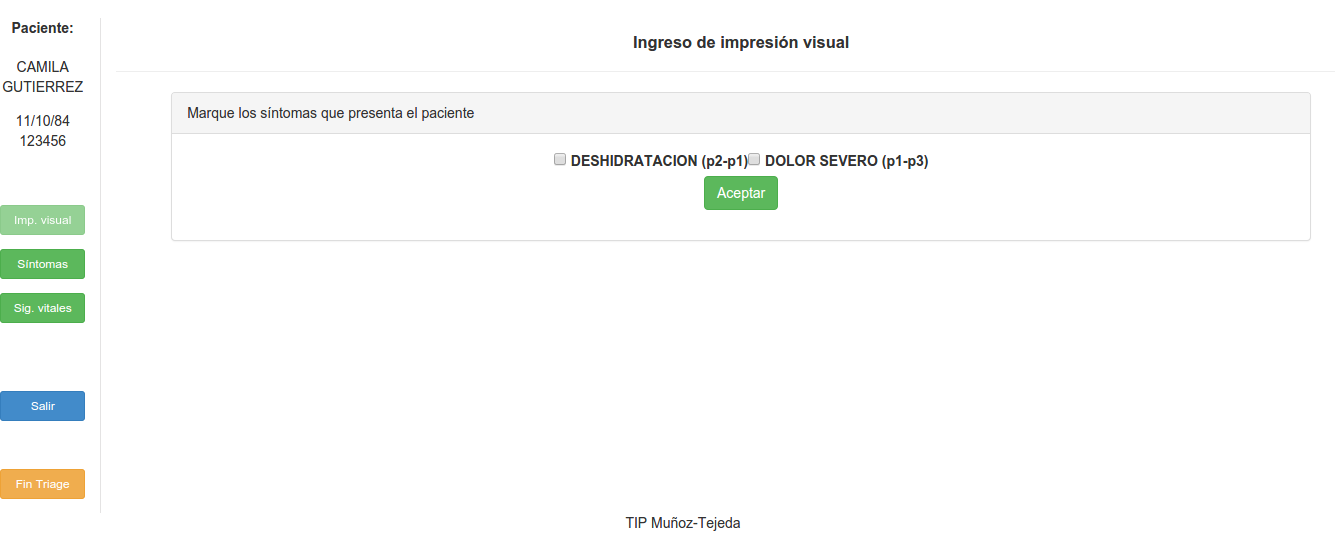
\includegraphics[width=0.99\textwidth]{impresion_visual.png}}
\caption{Pantalla inicial de Triage} \label{fig:triage_inicial}
\end{figure}
tiene una navegación definida por pestañas (que se pueden ver en la parte izquierda de la pantalla). Las pestañas permiten cambiar de pantalla de manera rápida y simple.

\subsection{Impresión Visual}
En la pestaña de impresión visual (figura \ref{fig:triage_inicial}) se cargan los síntomas que el enfermero/administrativo ve en el paciente que está siendo atendido. Una vez seleccionados los síntomas visuales, el usuario debe presionar el botón ``Aceptar''. En el caso de que un síntoma de Prioridad UNO sea seleccionado el sistema corta la interacción con el usuario con un cartel de confirmación (figura \ref{fig:impresion_visual_p1}).
\begin{figure}
\centerline{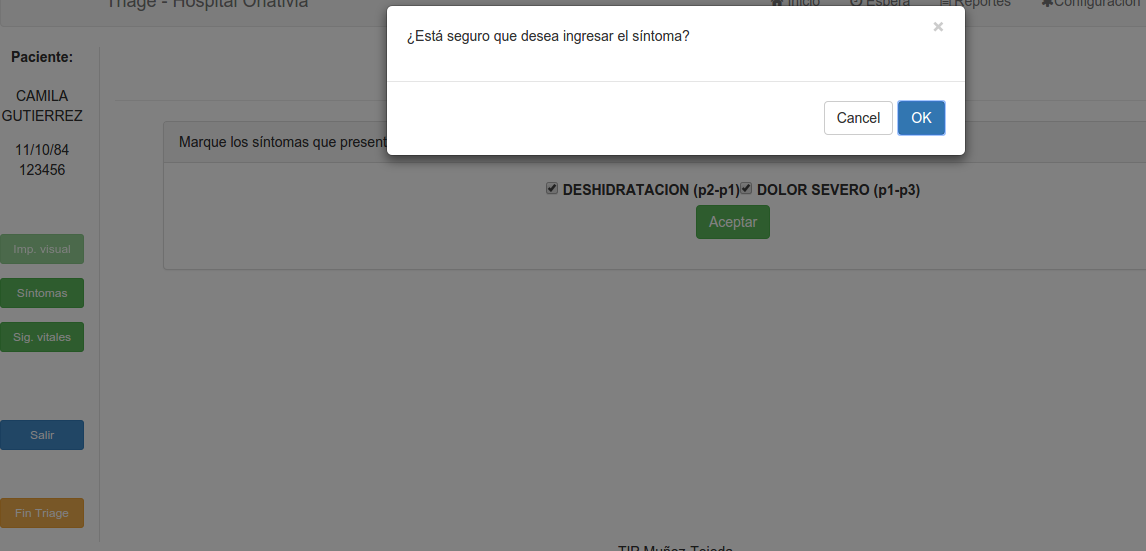
\includegraphics[width=0.99\textwidth]{impresion_visual_p1.png}}
\caption{Pantalla inicial de Triage} \label{fig:impresion_visual_p1}
\end{figure}
Si el usuario confirma, el sistema deriva directamente a la pantalla de Prioridad UNO, mostrando los datos y síntomas del paciente ingresado (figura \ref{fig:prioridad_uno}).
\begin{figure}
\centerline{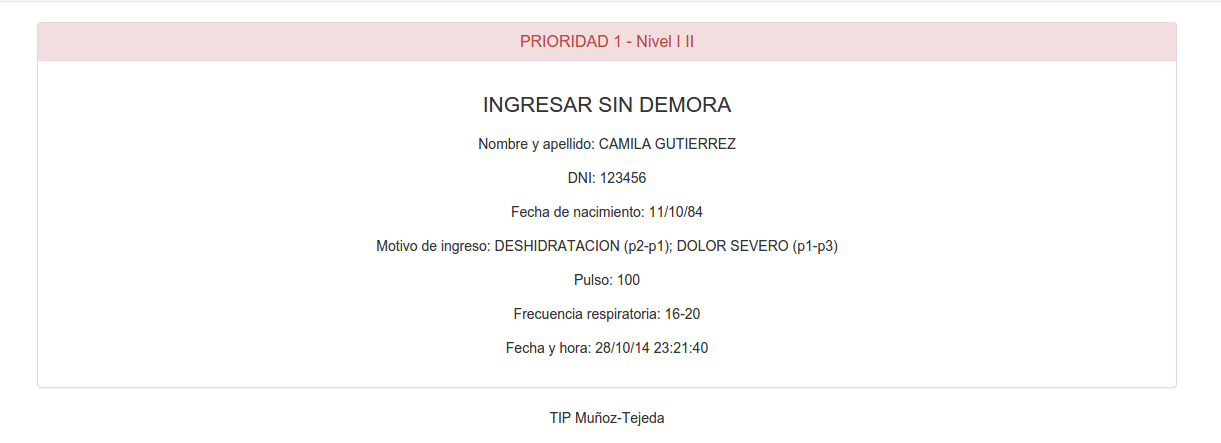
\includegraphics[width=0.99\textwidth]{prioridad_uno.png}}
\caption{Prioridad UNO} \label{fig:prioridad_uno}
\end{figure}

\subsection{Síntomas}
En la pestaña de síntomas (figura \ref{fig:sintomas})
\begin{figure}
\centerline{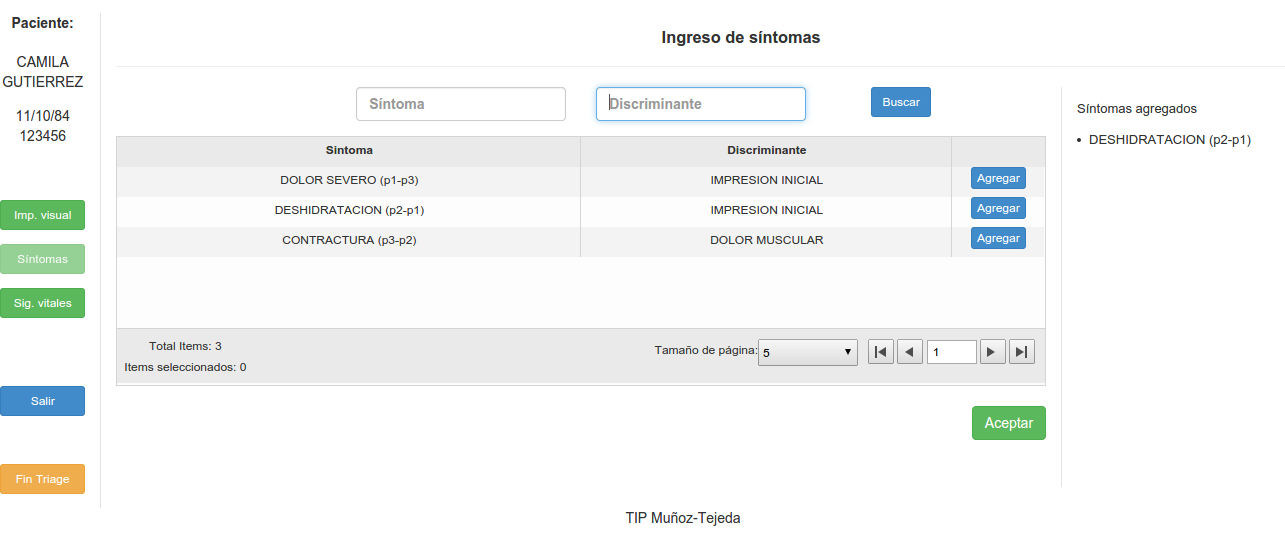
\includegraphics[width=0.99\textwidth]{sintomas.png}}
\caption{Pestaña de síntomas} \label{fig:sintomas}
\end{figure}
van a ser cargados los síntomas que el paciente informe. 

En el cuadro central se pueden ver todos los síntomas cargados en sistema, indicando cuál es su discriminante. Aquí se puede filtrar también por síntoma o discriminante (tal como se explica en la sección \ref{cap:filtrado_listado}) (Ver figura \ref{fig:sintomas_filtrar}).
\begin{figure}
\centerline{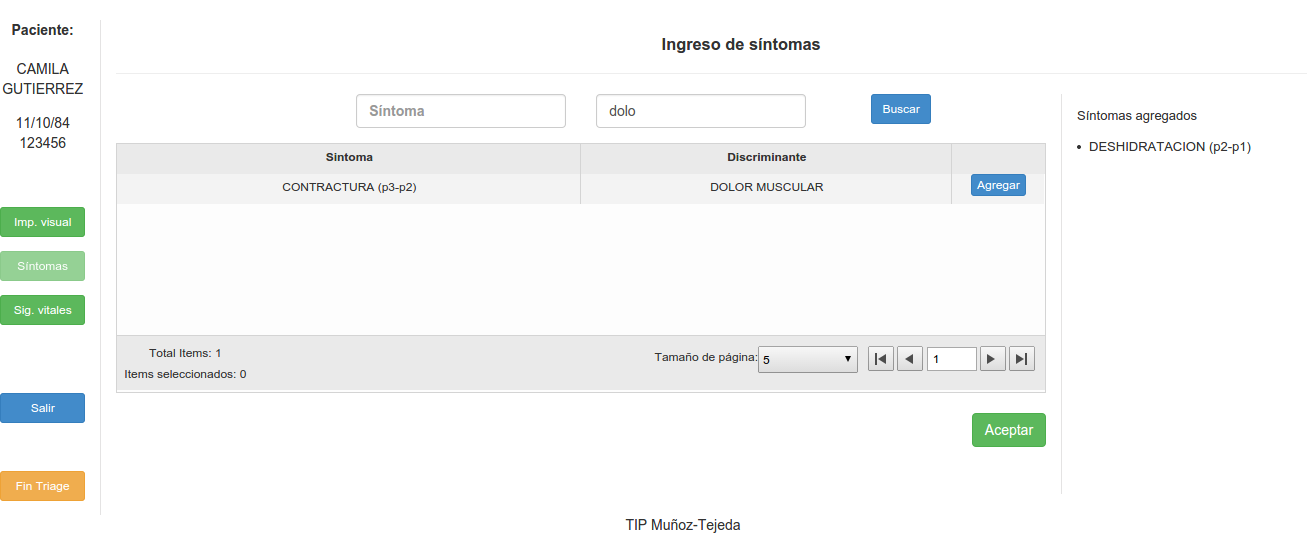
\includegraphics[width=0.99\textwidth]{sintomas_buscar.png}}
\caption{Filtrado en el cuadro de síntomas} \label{fig:sintomas_filtrar}
\end{figure}
Una vez filtrado el listado y encontrado lo que se busca, en cada fila del cuadro se puede ver el botón ``Agregar'' (figura \ref{fig:sintomas_agregar}), que permite cargar un nuevo síntoma al paciente.
\begin{figure}
\centerline{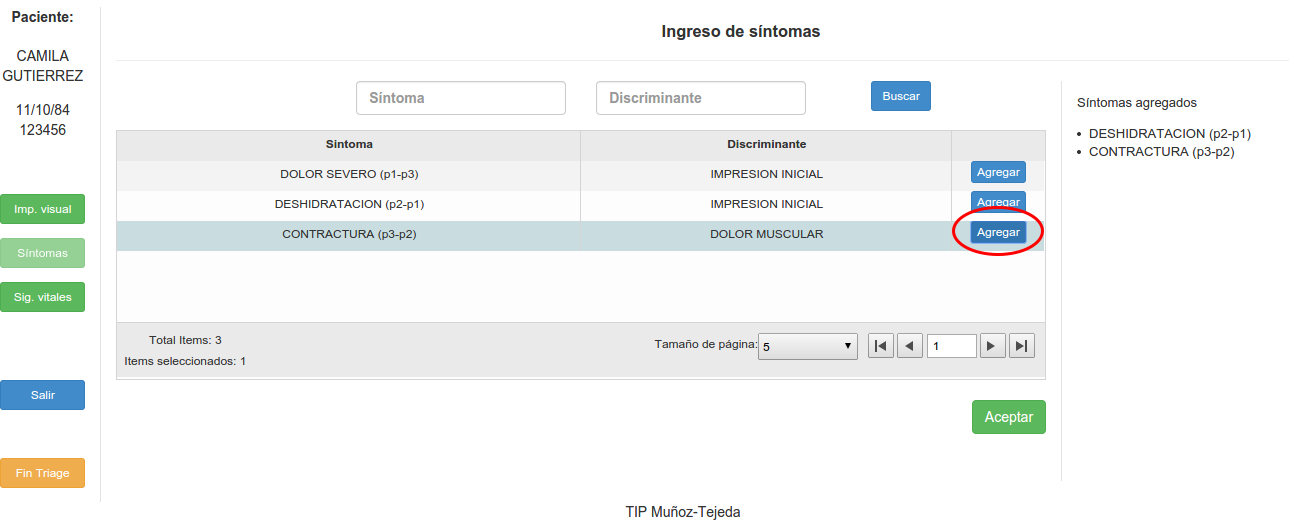
\includegraphics[width=0.99\textwidth]{sintomas_agregar.png}}
\caption{Agregar nuevo síntoma} \label{fig:sintomas_agregar}
\end{figure}
En la parte derecha de la pantalla se pueden ver los síntomas ya cargados. Se puede también eliminar algún síntoma agregado mediante el botón ``Borrar'' (que aparece al pararse con el puntero sobre el elemento a eliminar).

En el caso de ingresar un síntoma con Prioridad UNO,  el sistema corta la interacción con el usuario con un cartel de confirmación. Si el usuario confirma que efectivamente ese es el síntoma a agregar, el sistema deriva directamente a la pantalla de Prioridad UNO, mostrando los datos y síntomas del paciente ingresado (figura \ref{fig:prioridad_uno}).

Al finalizar con la carga, se debe presionar el botón ``Aceptar'' para grabar los síntomas seleccionados.


\subsection{Signos Vitales}
La tercer pestaña del Triage es para completar los signos vitales del paciente (figura \ref{fig:signos_vitales}).
\begin{figure}
\centerline{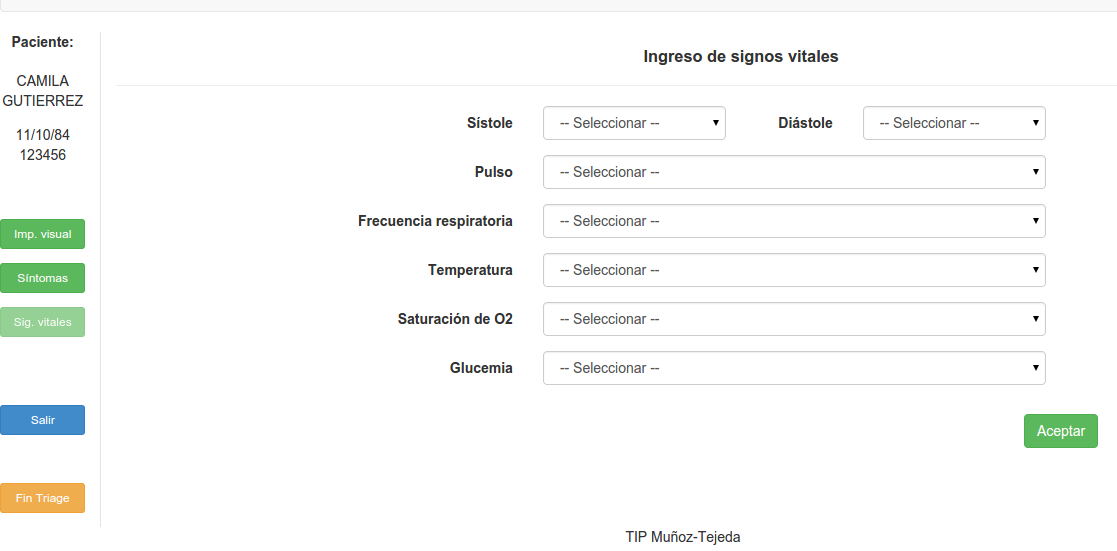
\includegraphics[width=0.99\textwidth]{signos_vitales.png}}
\caption{Signos Vitales} \label{fig:signos_vitales}
\end{figure}
Cada signo vital está definido para ser seleccionado de una lista acotada. En el caso de seleccionar algún valor que corresponda a una Prioridad UNO, el sistema mostrará un mensaje de confirmación. Si el usuario confirma la acción, se corta toda interacción mostrando la pantalla que indica atención inmediata (figura \ref{fig:prioridad_uno}).

Al finalizar de cargar los signos vitales, se debe presionar el botón ``Aceptar'' (figura \ref{fig:signos_vitales_guardar})
\begin{figure}
\centerline{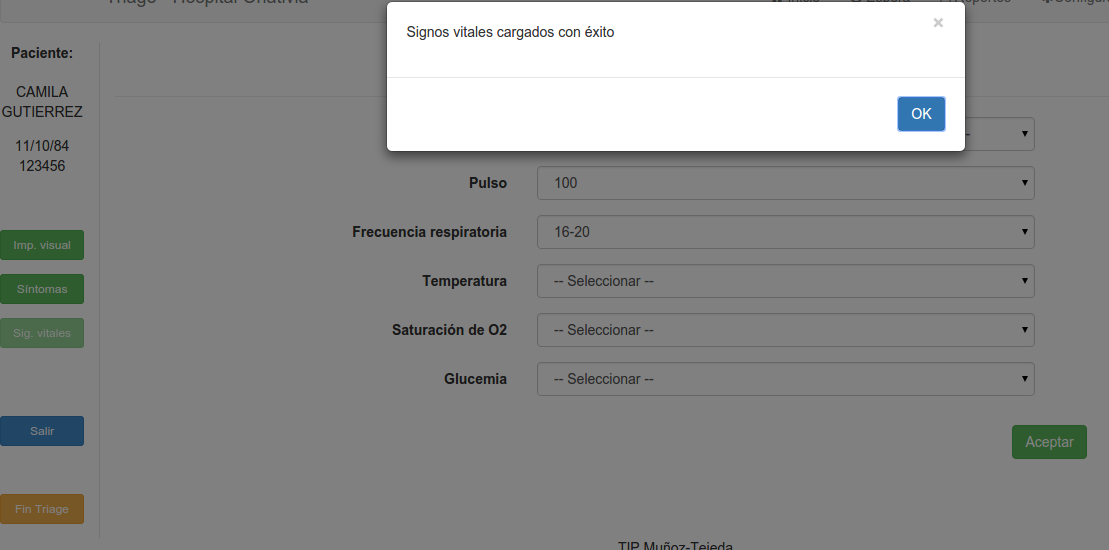
\includegraphics[width=0.99\textwidth]{signos_vitales_guardar.png}}
\caption{Signos Vitales} \label{fig:signos_vitales_guardar}
\end{figure}
y el sistema informará que los datos se han guardado con éxito.


\subsection{Fin de la carga}
Al terminar de cargar los síntomas hay dos caminos:
\begin{description}
\item[Finalizar Triage]  \mbox{} \\
Para finalizar el Triage, se debe presionar el botón sobre la pestaña izquieda llamado ``Fin Triage'' (figura \ref{fig:fin_triage}).
\begin{figure}
\centerline{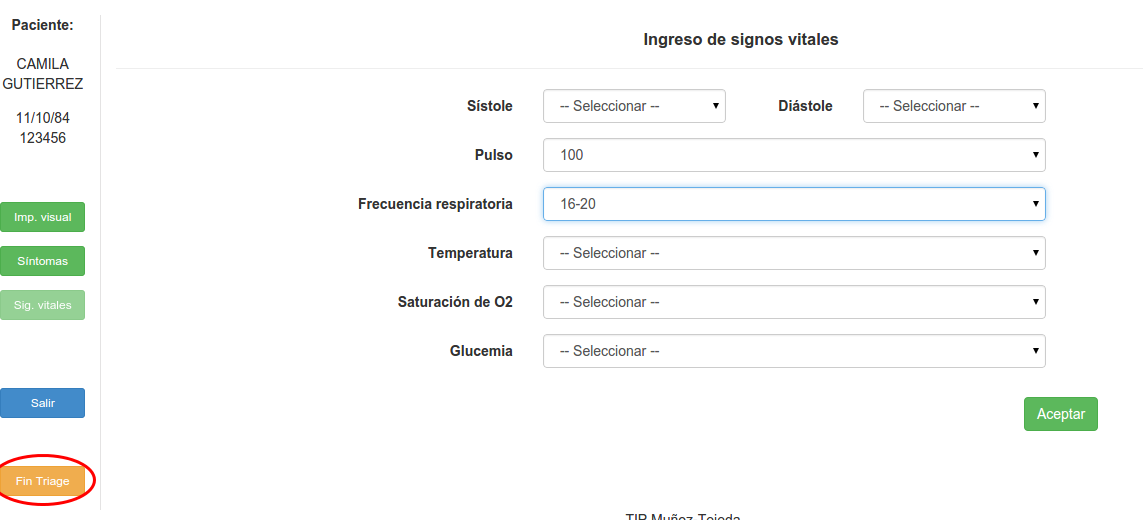
\includegraphics[width=0.99\textwidth]{fin_triage.png}}
\caption{Fin Triage} \label{fig:fin_triage}
\end{figure}
 Al hacer esto, el sistema calcula la prioridad del paciente, indicando todos los síntomas cargados y sus datos personales. 

Esta acción sólo puede mostrar las pantallas de Prioridad DOS (figura \ref{fig:prioridad_dos}) 
\begin{figure}
\centerline{
\includegraphics[width=0.99\textwidth]{prioridad_dos.png}}
\caption{Prioridad DOS} \label{fig:prioridad_dos}
\end{figure}
y Prioridad TRES (figura \ref{fig:prioridad_tres}), 
\begin{figure}
\centerline{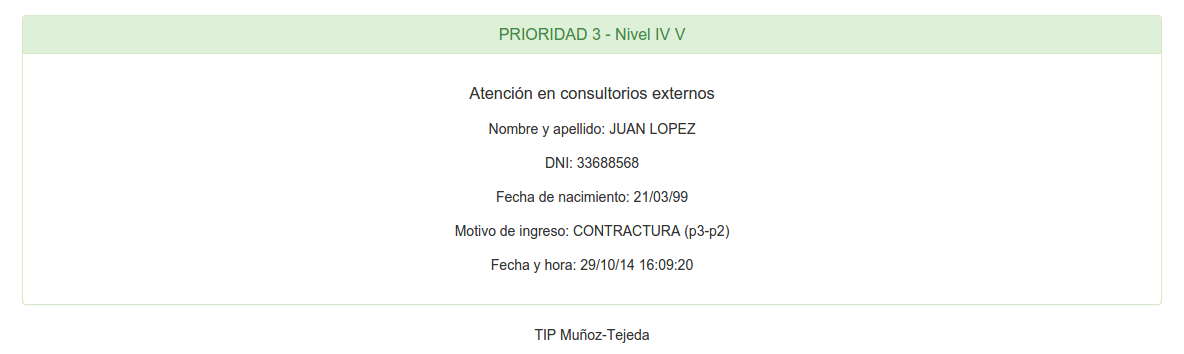
\includegraphics[width=0.99\textwidth]{prioridad_tres.png}}
\caption{Prioridad TRES} \label{fig:prioridad_tres}
\end{figure}
ya que la pantalla de Prioridad UNO sólo se presenta al seleccionar un síntoma de Prioridad UNO y corta toda interacción con el usuario.
Finalizar el Triage no quita al paciente de la lista de espera, simplemente calcula su prioridad. 

\item[Salir de la carga]\mbox{} \\
En el caso de querer abandonar la carga de síntomas para poder retomarla más tarde, el sistema provee la acción ``Salir'' (figura \ref{fig:fin}),
\begin{figure}
\centerline{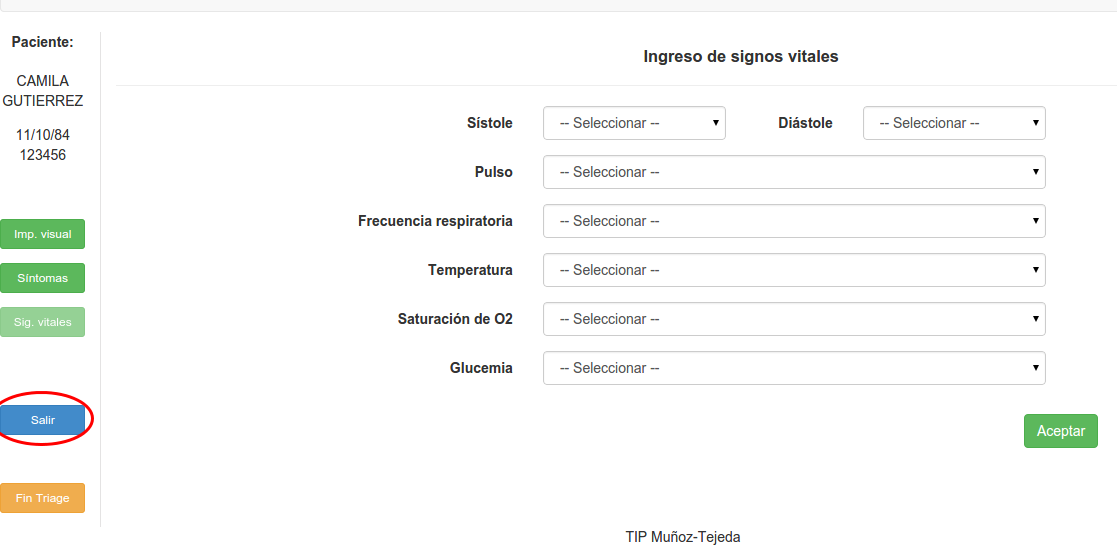
\includegraphics[width=0.99\textwidth]{fin.png}}
\caption{Salir de la carga} \label{fig:fin}
\end{figure}
que permite guardar los síntomas ingresados hasta el momento y poder recuperarlos si se carga el paciente desde la lista de espera.


\end{description}